% arara: xelatex
% arara: xelatex
% arara: xelatex

% options:
% thesis=B bachelor's thesis
% thesis=M master's thesis
% czech thesis in Czech language
% english thesis in English language
% hidelinks remove colour boxes around hyperlinks

\documentclass[thesis=M,english]{FITthesis}[2019/12/23]

\usepackage[utf8]{inputenc}
\usepackage{amsmath} %advanced maths
\usepackage{amssymb} %additional math symbols
\usepackage{lipsum,tikz}
\usepackage[cache=false, outputdir=out]{minted}
\usepackage{listings} % typesetting of sources
\usepackage[fontsize=11pt]{fontsize}
\usepackage{xcolor}
\usepackage{float}
\usepackage{fancyvrb}

\definecolor{codegreen}{rgb}{0,0.6,0}
\definecolor{codegray}{rgb}{0.5,0.5,0.5}
\definecolor{codepurple}{rgb}{0.58,0,0.82}
\definecolor{backcolour}{rgb}{0.95,0.95,0.92}

\lstdefinestyle{mystyle}{
    commentstyle=\color{codegreen},
    keywordstyle=\color{magenta},
    numberstyle=\tiny\color{codegray},
    stringstyle=\color{codepurple},
    basicstyle=\ttfamily\footnotesize,
    breakatwhitespace=false,
    breaklines=true,
    captionpos=b,
    keepspaces=true,
    showspaces=false,
    showstringspaces=false,
    showtabs=false,
    tabsize=4
}

\lstset{style=mystyle}

\usepackage{dirtree} %directory tree visualisation

% tikz thingies
\newcommand\todo[1]{\textcolor{red}{#1}}
\usetikzlibrary{calc,positioning,arrows,shapes.geometric}
\tikzstyle{process} = [rectangle, 
minimum width=3cm, 
minimum height=1cm, 
text centered, 
text width=3cm, 
draw=black, 
]

\usetikzlibrary{arrows.meta}
\tikzset{>={Latex[width=3mm,length=3mm]}}

% list of acronyms
% \usepackage[acronym,nonumberlist,toc,numberedsection=autolabel,nomain]{glossaries}
\iflanguage{czech}{\renewcommand*{\acronymname}{Seznam použitých zkratek}}{}
% \makeglossaries

\newcommand{\tg}{\mathop{\mathrm{tg}}} %cesky tangens
\newcommand{\cotg}{\mathop{\mathrm{cotg}}} %cesky cotangens

% % % % % % % % % % % % % % % % % % % % % % % % % % % % % % % % % % % 
% % % % % % % % % % % % % % % % % % % % % % % % % % % % % % % % % % % 
\department{Department of theoretical computer science}
\title{Tiny86 Debugger}
\authorGN{Filip} %author's given name/names
\authorFN{Gregor} %author's surname
\authorWithDegrees{Bc. Filip Gregor} %author's name with academic degrees
\author{Filip Gregor} %author's name without academic degrees
\supervisor{Ing. Petr Máj}

\acknowledgements{First and foremost, a thanks to my parents, who has always
supported me and enabled my to pursue my dreams, whatever they may be. I would
also like to thank to my supervisor, who spent an ungodly amount of time and
patience to break through my stuborness and make this thesis what it is. Last
but not least, a thanks to my girlfriend, without her this work would never come
to be.}

\abstractCS{Abstrakt v cestine}
\abstractEN{Abstract In english.}

\placeForDeclarationOfAuthenticity{Prague} %where you have signed the declaration
\keywordsCS{Debugging, Debugger, Debug, Compiler.}
\keywordsEN{Debugging, Debugger, Debug, Compiler.}
\declarationOfAuthenticityOption{4} %select as appropriate, according to the desired license
\website{https://github.com/Gregofi/thesis-monorepo}

\begin{document}

% \newacronym{LZW}{LZW}{Lempel Ziv Welch}
% \newacronym{RLE}{RLE}{Run-Length Encoding}

\chapter{Introduction}
Computers has many components that allows it to function. One of the most integral one is processor.
This component does all the calculations that computer needs to do. However, processors can only understand
zeros and ones. Those sequences of zeroes and ones (called machine code) makes up a program that the processor can execute.
They can also save the results of their calculations, for this the computer
has a memory, but writing and reading from it can be slow. Fortunately, \textit{registers} come to
the rescue! They are part of the processor itself and so it has very fast access to them, but unfortunately,
there are only few of them.

As we said, processors can only understand machine code. But writing those sequences of zeros and ones and understanding
what they do is very hard for human programmer. Because of this, a text mapping was created,
called \textit{assembly language}. See the example on figure \ref{fig:assembly-example}.
This is certainly more readable than binary, but is ugly nonetheless\footnote{At least for normal mortal. Some of us enjoy reading such monstrosities.}.
For example the \texttt{MOV EAX, 1} instruction moves value $1$ to the register named \texttt{EAX}.

\begin{figure}\label{fig:assembly-example}
\begin{lstlisting}
PROC:
    PUSH    EBP
    MOV     EBP, ESP
    CMP     [EBP + 8], 0
    JLE     LN2
    MOV     EAX, 1
    JMP     LN1
LN2:
    XOR     EAX, EAX
LN1:
    POP     EBP
    RET
\end{lstlisting}
\caption{Example of assembly language}
\end{figure}

Programs are executed from top to bottom sequentially, instruction by instruction. But certain instructions can change this control flow. For example the instruction \texttt{JMP dest}
jumps to a label (\texttt{LN1} in the example) and the execution continues from there. This allows the program to repeat or skip some part of the code.
Notice the JLE instruction. This instruction performs mentioned jump but only if certain other condition holds true.
These instructions can make it harder for programmer to follow the control flow \cite{gotobad}.

Because writing and reading assembly was a pain, higher level programming languages were created.
Aim of these languages is to abstract away the details of a computer. One of the older languages is the C programming language (1972).
Example of a program in C is seen on figure \ref{fig:c-positive}, this program does the same thing as the assembly one on figure \ref{fig:assembly-example}.

\begin{figure}\label{fig:c-positive}
\begin{minted}{C}
int positive(int n) {
    if (n > 0) {
        return 1;
    } else {
        return 0;
    }
}
\end{minted}
\caption{C function that checks if number is positive.}
\end{figure}

With C, knowing about the internals of the computer is no longer needed.
We do not store values into registers, instead they are kept in variables. We can use conditional statements,
which are more concise than using jumps \cite{gotobad}.
The functions and variables themselves also have names from which
can be apparent what is the purpose of it contrast to register names like \texttt{EAX}.

However, upon deeper inspection of the language, it does not abstract away everything. C has a feature called
\textit{pointers}. Those are special kind of variables which points into the computer memory\footnote{On modern OS,
a concept named \textit{virtual memory} is used. This maps addresses used by process to physical memory.
Pointer values are virtual memory addresses. See \cite{modern-os}.}.
So C does not necessarily abstract everything away. That can sometimes be a good thing, because if you need to
interact with the computer hardware you don't have to resort to assembly, but can use C. For example the Linux
Kernel is written mostly in C \cite{linux-source}. Over the years, many programming languages came to be, and
some are more abstract than others. For example language Python doesn't have pointers like C.

However, we previously said that processors can only understand machine code and high level languages are certainly not machine code.
We need to translate the language into assembly, and this is how \textit{compilers} came to be. Compiler is a program
that reads some source code of high level language and produces assembly for the processor to understand. Compilers
are very complicated piece of software, and we will talk about them in detail in chapter \todo{Debugging - Compiler support}.
For now, just keep in mind that the source code needs to be someway translated and that the computer cannot
run the source code of high level language directly.

\begin{figure}[H]\label{fig:binary-search}
    \begin{minted}{c}
int binary_search(int* arr, int len, int n) {
    int lo = 0;
    int hi = len;
    while (lo < hi) {
        int i = (lo + hi)/2;
        if (arr[i] < n) {
            lo = i;
        } else if (arr[i] > n) {
            hi = i;
        } else {
            return 1;
        }
    }
    return 0;
}
    \end{minted}
    \caption{Binary search algorithm in C language.}
\end{figure}

On the \ref{fig:binary-search} figure we present more complicated example of a program written in high level programming language. This
is an implementation of the binary search algorithm. It operates on sorted sequence of numbers and checks
if there is some concrete number contained. This algorithm is widely implemented in many standard libraries \todo{Citace}.

\section{Debugging}
Programs are mostly written by humans, and humans tend to make mistakes \cite{human-error}.
We are no exception, as we have also made a mistake in the program that implements binary search.
Lets try to run the program with a \texttt{[1,2,3]} sequence and search for number $4$. This
number is apparently not in the sequence, so expected output would be $0$. Instead, the program would run forever,
because of a mistake we have made in the source code. We will call such mistakes
a \textit{bug}\footnote{The term \textit{bug} actually comes from a real bug that got stuck in relays back when it was a critical part of cumputers.
They literally had to debug the machine by taking the bug out.}.

Well, now we have to find out where the error is. We could just try to look at the source code and
find the mistake this way. This is a valid strategy, here we could probably
figure out that the condition \texttt{lo < hi} never comes to be, since where else could we get
stuck in an infinite loop? Now, it would be helpful if we could see the states of \texttt{lo} and
\texttt{hi} in each iteration of the cycle. We could resort to print statements, but that can
quickly get overwhelming, especially in infinite loop. Not to mention we need to recompile
the program if we want to print something different. All is not lost, a special
piece of a program was created specifically for this purpose, called a \textit{debugger}.
Debugger is a program which can inspect another program. They often have complete control of the program.
The program being debugged will be called a \textit{debugee}.

Debugger is able to inspect the state of the debugee, like values of its variables. Debugger is also able to control
the flow of the program. They allow \textit{breakpoints} to be set at each line of the source code\footnote{Advanced debuggers allows breakpoints to be set inside expressions.
This is especially important for functional languages, as their functions often consists of one big expression.}.
When the program is about to execute the line of code with the breakpoint, the control is passed back to the
debugger and user can inspect the state of the program at that line. There are also conditional breakpoints,
which only triggers when some condition holds (for example the value of variable \texttt{i} must be equal to zero).

Finally, debuggers also allow \textit{stepping}. This also modifies the control flow of the program.
\begin{itemize}
    \item \textit{step in} - Executes current statement and stops on the next one. If current statement is a function call then
                    it will be executed and program will be paused on the first statement in that function.
    \item \textit{step over} - Same as step in, but if current statement is a function call then the program will
                      be paused on the next statement after the call.
    \item \textit{step out} -  Executes as much as needed to return from current function. Stops on next statement that
                      should be executed after the function returns.
\end{itemize}

Now, back to our program. Lets put a breakpoint on line $8$, after $i$ is being set. We will monitor how the \texttt{lo} and \texttt{hi}
changes. If you run the program with debugger attached, you will see output similar to what is displayed on figure \ref{fig:lldb-debug1}.
Here, you can see the line on which the execution was stopped. It is also possible to print the state of variables. In each loop,
you can print the value of variable and then continue execution until another breakpoint. There is only one set, so the execution will
again be stopped on line $8$. The value of \texttt{hi} will not change, which is expected. Value of \texttt{lo} will gain following values:
$0$, $1$, $2$, $2$, $2$ and the trend continues. The value of variable $i$ is computed as $i = (\text{lo} + \text{hi})/2 = (2 + 3)/2 = 2$,
because division in C rounds the value down. The fix is to change the
line $9$ to \texttt{lo = i + 1}. With the debugger, it was simple to find out what was happening.

\begin{figure}\label{fig:lldb-debug1}
\begin{minted}{c}
   5   	    int hi = len;
   6   	    while (lo < hi) {
   7   	        int i = (lo + hi)/2;
-> 8   	        if (arr[i] < n) {
   9   	            lo = i;
   10  	        } else if (arr[i] > n) {
   11  	            hi = i;
Target 0: (a.out) stopped.
(lldb) p lo
(int) $0 = 0
(lldb) p hi
(int) $1 = 3
\end{minted}
\caption{Example of debugging a program in LLDB debugger.}
\end{figure}

We previously said that processors themselves only understand machine code. So how it is possible that we can debug the program and the debugger knows about lines, variables etc. when the program itself is just machine code. The compiler has to lend a hand here. It embeds information about the source code. For example, it maps lines of source code to machine code instructions. Thanks to this mapping, the debugger knows that line $x$ corresponds to instruction $y$ in the machine code, and can put breakpoint there.
If the compiler doesn't emit any information into the executable the debugger would only work with assembly, as seen on figure \ref{fig:lldb-debug2}. This
is a lot more discomforting than debugging source code directly.

\begin{figure}\label{fig:lldb-debug2}
\begin{lstlisting}
->  0x100003e3c <+112>: b      0x100003e78               ; <+172>
    0x100003e40 <+116>: ldr    x8, [sp, #0x20]
    0x100003e44 <+120>: ldrsw  x9, [sp, #0xc]
    0x100003e48 <+124>: ldr    w8, [x8, x9, lsl #2]
\end{lstlisting}
\caption{Example of debugging a program in LLDB debugger without debugging information.}
\end{figure}

\section{Teaching compilers}
Many schools about computer science have compiler course. At Faculty of Information Technologies, there is one too, called \textit{Code Generators} (NI-GEN). In this course, student is tasked to build a simple compiler for a C like language. The target of the compiler is Tiny86 (T86) architecture. This architecture \todo{Never mentioned any architectures before} does not have a processor that can execute it, instead a virtual machine (or interpreter, if you will) was created for it. The architecture is supposed to ease the code generation and let the students focus on the more interesting parts of the compiler, like register allocation or optimization, instead of the nitty gritty detail of x86 (or different architecture, should the students choose it).

There is however a problem with using T86, there is no debugger that supports it. So if a compiler of some student generates code badly, it takes a non-trivial amount of effort to find the error. T86 offers some very light debugging capabilities, but they are very far from real debugging. Also, compiling debugging informations is not taught at all in the NI-GEN course. If a debugger was provided to the students, it might be incetiving to compile such information to ease their lives later, when they will need to find errors in their compilers which will inevitably happen. This way they will also learn how and what information the compiler needs to embed for the debugger to work.

\section{Goals of the thesis}
The primary goal is to create a debugger for the T86 virtual machine which allows to debug both on the machine code level and at the source code level. The debugger should be extensible enough to work with intermediate representation also. The debugger should be similar to real world debuggers, in terms of how it works. This will require non-trivial changes in the T86 virtual machine source code. The students compilers will also have to generate debugging information. Format of the debugging information should be so that it is not discouraging for students to generate.

\section{Structure of the thesis}
\begin{enumerate}
    \item The \textit{Introduction} describes the motivation behind the thesis and basic terms with which should the reader be familiar.
    \item \textit{Debuggers - On the Shoulders of Giants} describes how are debuggers implemented and what support is needed on various levels (OS, processors, compilers) for them to work.
    \item \textit{T86 Virtual Machine} describes the T86 architecture and how are some of the parts implemented.
    \item \textit{Implementation} describes how the implementation is done. It is divided into three main parts, first is what changes and additions were necessary to the T86 VM. Then it is described how the debugger itself is implemented. Finally, a proof of concept compiler is created to demonstrate how the debugger works and that it is indeed simple to generate debugging information for it.
    \item \textit{Conclusions} summarizes the result of the thesis and speaks of possible future work.
\end{enumerate}


\chapter{Debugging support}

\begin{quote}
  \textit{Debugging is twice as hard as writing the code in the first place. Therefore, if you write the code as cleverly as possible, you are, by definition, not smart enough to debug it.}\begin{flushright}
    \tiny{Brian W. Kernighan}
  \end{flushright}
\end{quote}

We already mentioned in the first chapter that to debug programs written in
high level programming languages, we need the compiler to emit debugging
information. But debugging support must also be provided by operating system
(if there is one) and by processor itself. However, we can still debug programs
in machine code. We briefly mentioned this in chapter 1 \todo{ref}, however, we
won't see source code, but only assembly. This can still be useful, for example
for reverse engineering. And, as was already hinted, source level debugging is
built upon assembly debugging. In this chapter, we will describe on which
levels must assembly level debugging be supported. Additionaly, we'll discuss
how are compilers and debuggers able to allows us to debug source code
althrough the programs are still machine code programs. 

\section{Support on CPU level} In first chapter it was said that CPU can only
execute machine code which is made of instructions and that it has certain
registers. Which instructions and registers the CPU has can differ from CPU to
CPU. This is specified by \textit{Instruction Set Architecture} (ISA)
\cite{aps-isa}. It is an abstract interface between the hardware and lowest
level software (machine code). It contains all information needed to write a
program in machine code. In general, ISA specifies following: 
\begin{itemize}
    \item Set of machine code instructions - Specifies instructions the ISA has
          and what operands each instruction has.
    \item Register set - Which
          registers the ISA has\footnote{Strictly speaking ISA doesn't have
          to use registers. It's possible to use only stack or accumulator,
          but most used ISAs use registers, so we'll ignore those
          architectures. }.   
    \item Addressing modes - Possible methods to refer to memory or register. 
\end{itemize} There are other specification,
however they are not relevant to this thesis. For each instruction and operand
there is specified how they should be encoded into binary (remember, that's
what the CPU can understand). CPU then \textit{implements} some ISA. If two
different CPUs implements the same ISA then they should be able to run the same
machine code program. For example, most PC use the \textit{x86} architecture
\cite{aps-isa}, althrough the ARM architecture is also seeing use in personal
computers, for example the Apple Sillicon is of ARM architecture.

The x86 architecture is so called \textit{Complex Instruction Set Architecture}
(CISC). It contains many instructions that do many things at once, have varying
length and takes multiple clock cycles to complete \cite{intel-manual}. On the
other hand the ARM architecture is \textit{Reduced Instruction Set
Architecture} (RISC). The number of instructions is smaller, they are intended
to be small building blocks from which complex operations may be created by
using many of them. Each instruction in RISC also has same length. Both
architectures have their pros and cons, althrough some literature suggest that
in modern days the choice of architecture is irrelevant if one is only
considering performance and power
consuption  \cite{riscvscisc1, riscvscisc2}. Unless specified otherwise the
rest of this chapter will be talking about x86. This is because T86 \todo{ref}
is loosely based on x86, so it is most relevant for us.

In first chapter we briefly mentioned that machine code programs can instead be
written in Assembly language. Assembly is almost 1:1 mapping to machine code.
When showing programs, we will show them in assembly. In figure
\ref{fig:assembly-example2}, we present another example of a program that was
compiled from C to assembly of the x86 architecture. As seen, instructions have
various operands. Most often registers (\texttt{RBP, RSP, EAX}), memory
(\texttt{[rbp-4]} is reference to memory at address which is in register
\texttt{rbp} minus $4$), or labels (like \texttt{L2}). Labels are not part of
machine code, instead memory address has to be provided. This is a small part
where assembly and machine code differ. For detailed overview of the x86
instructions see \cite{intel-manual}.

\begin{figure}\label{fig:assembly-example2}
    \begin{lstlisting}
max:
    push    rbp
    mov     rbp, rsp
    mov     QWORD PTR [rbp-24], rdi
    mov     DWORD PTR [rbp-28], esi
    mov     rax, QWORD PTR [rbp-24]
    mov     eax, DWORD PTR [rax]
    mov     DWORD PTR [rbp-4], eax
    mov     DWORD PTR [rbp-8], 1
    jmp     .L2
.L3:
    mov     eax, DWORD PTR [rbp-8]
    cdqe
    lea     rdx, [0+rax*4]
    mov     rax, QWORD PTR [rbp-24]
    add     rax, rdx
    mov     eax, DWORD PTR [rax]
    cmp     DWORD PTR [rbp-4], eax
    cmovge  eax, DWORD PTR [rbp-4]
    mov     DWORD PTR [rbp-4], eax
    add     DWORD PTR [rbp-8], 1
.L2:
    mov     eax, DWORD PTR [rbp-8]
    cmp     eax, DWORD PTR [rbp-28]
    jl      .L3
    mov     eax, DWORD PTR [rbp-4]
    pop     rbp
    ret
    \end{lstlisting}
    \caption{Compiled C program with GCC 9.4 compiler as x86 assembly.}
\end{figure}

\subsection{Registers}

The x86 architecture has a set of general purpose registers.
Some of these are
\begin{itemize}
    \item RAX - Accumulator for operands and results data,
    \item RCX - Counter for string and loop operations,
    \item RSP - Stack pointer,
    \item RBP - Pointer to data on the stack.
\end{itemize}
The names and number of general purpose registers change based on bit mode. 64-bit (also named x86-64) mode has 16 of them, while 32-bit has 8.
Althrough the \texttt{RSP} and \texttt{RBP} are called general purpose they are often only used for pointing at the top of the stack,
resp. to the base of the stack. Stack is special part of program memory, it mostly has LIFO
semantics\footnote{For example the \texttt{mov eax, DWORD PTR [rbp - 4]} does not respect
LIFO semantics, because it reads directly from the stack and not from the top.}
It can be used to store intermediate result, arguments to functions, return address etc.
This register is weird in a sense that it has this very special purpose but is still considered part of
the general purpose registers~\cite{intel-manual}. One might use it for storing calculations, but it would make
rest of the instructions that work with stack behave unexpectedly.

Instruction pointer register (RIP on x86-64, EIP on x86) contains address of the current instruction to be executed. As we mentioned
in Introduction \todo{ref}, programs are executed sequentially from top to bottom, with certain instructions
having the ability to change the control flow. When an instruction get executed, the size of the instruction
will be added to the value in RIP register. This will advance the instruction pointer to the next instruction.
Or, if the instruction changes control flow, the value in instruction pointer will be changed to the destination
of the instruction. The register can also be changed directly.

Another interesting register is the \texttt{EFLAGS} register. The register contains group
of flags, which can alter various behavior of the CPU, or the CPU itself sets them
as result of some instruction. For example the instruction \texttt{cmp} compares its two operands
and if they are the same the \textit{zero} flag in the \texttt{EFLAGS} register will be set.

\subsection{Interrupts}
Interrupt is a special request to the CPU to stop execution of current program
and to quickly react to the reason that caused the request
\cite{aps-interrupts}. Example of such event can be keyboard press or error in
an program (division by zero). There are two main categories
\cite{intel-manual}
\begin{itemize}
    \item An \textbf{interrupt} is an asynchronous\footnote{Meaning that the
    interrupt may happen when another instruction is being processed (not on
the CPU clock edge).} event that is typically triggered by an Input/Output (IO)
device. \item An \textbf{exception}\footnote{Unfortunately, this term will
    become quite overloaded in this thesis.} is a synchronous event that is
        generated when the processor detects one or more predefined conditions
        when executing an instruction. These are further divided into three
        classes: faults, traps and aborts.
\end{itemize}

When an interrupt or exception happens, the processor halts execution of
current program and switches to specific interrupt handler. Interrupt handler
is just another sequence of instructions that handles the interrupt. Example of
an exception is the \texttt{INT3} instruction. When this instruction is
executed an interrupt is generated. This instruction is specifically meant to
be used as a breakpoint. We can supply code that will be responsible for
handling the breakpoint as the interrupt handler. However, on modern PCs a
Operating System (OS) is governing the PC. Alas, we cannot touch the interrupt
handler directly. Instead, an OS is going to have to provide another layer of
support for debugging.

Recall the EFLAGS register mentioned in section \ref{X}. There is a special
flag called trap flag. When it is set, cpu will issue an interrupt after every
executed instruction. This could be useful if we wanted to inspect execution
instruction by instruction.

\todo{Debugging embedded}

\section{Operating system support} Operating system is a layer between computer
components (cpu, memory, input/output devices, \dots) and software. It is
responsible for handling all those resources so programmers do not have to
think about it \cite{modern-os, os-concepts}. Managing resources is not only to
make writing programs easier, but to make sure that they are safe from each
other. Modern operating system allows to run multiple programs at once (or at
least offer the illusion that it can) and they make sure that one program
cannot overwrite data or otherwise interfere with other programs. Normal
programs runs in so called \textit{user space}, which has limited capabilites.
Kernel on the other hand runs in \textit{kernel space}. It has full access to
hardware of the computer, can use all instructions, can permit or mask
interrupts and so on.

However, if programs were limited to user space all the time they would be very
limited. Sometimes, they need to escape the confiment of the OS, for example to
read a file or communicate with other processes. Operating systems provide an
interface through which the user space program can leverage small part of the
kernel - system calls. They offer a way of requiring some service from the OS.
This API is often in form of C and C++ functions~\cite{os-concepts}. A part of
these functions is a special instruction, like \texttt{SYSCALL} on
x86~\cite{intel-manual}, that switches the mode to kernel space. The kernel has
to check if the call is correct, since it will be executed in kernel space with
full access.

The most prelevant operating systems today are Microsoft Windows, Linux and MacOS.
Linux and MacOS systems are somewhat similar, but Windows is very different.

\subsection{Linux}
Linux offers special system call which is very handy for debugging. It is
called \texttt{ptrace} \cite{ptrace} - process trace. It has following
signature: \texttt{ptrace(PTRACE\_COMMAND, pid, ...)}. It takes a
\texttt{PTRACE\_COMMAND}, which specifies the behaviour of the function (for
example \texttt{PTRACE\_SINGLESTEP} for single step), pid of some process and
some other parameters, depending on the \texttt{PTRACE\_COMMAND} that was
chosen. It allows to observe and control the execution of another process, this
process will be the debugee. In the context of \texttt{ptrace}, we will instead
use the word tracee for the debugee, and tracer for the debugger, to be
consistent with ptrace documentation.

\texttt{ptrace} has many commands, here are some of the most important:
\begin{itemize}
    \item \texttt{PTRACE\_PEEKTEXT, PTRACE\_PEEKDATA} - Read tracee's memory,
    \item \texttt{PTRACE\_POKETEXT, PTRACE\_POKEDATA} - Write into tracee's memory,
    \item \texttt{PTRACE\_GETREGS} - Read tracee's register values,
    \item \texttt{PTRACE\_SETREGSET} - Modify tracee's register values,
    \item \texttt{PTRACE\_GETSIGINFO} - Retrieve information about the signal that caused tracee to stop,
    \item \texttt{PTRACE\_CONT} - Restart the stopped tracee process,
    \item \texttt{PTRACE\_SINGLESTEP} - Restart the stopped tracee but
          stop it after executing one instruction.
\end{itemize}

Linux however needs some way of notifying the debugger that the tracee
encountered a breakpoint, or that some other event requiring debugger attention
happened. To this end, \textit{signals} are used. They are in principle similar
to CPU interrupts. They are however on the OS level. A signal is used in UNIX
and Linux systems to notify a process that a particular event has occured
\cite{os-concepts}. Signals can be sent to processes. When such process
receives a signal, it stops its execution and starts the execution of a signal
handler. There are various signal types. Most signals can have custom signal
handler defined by the process. If no handler is defined then a default one is
provided by the OS. However handlers for \texttt{SIGKILL} and \texttt{SIGSTOP}
cannot be changed \cite{signals}.

Reason for rising a signal can be \todo{Tady toho asi bude vic}
\begin{itemize}
    \item CPU Interrupt (Division by zero, Breakpoint hit),
    \item System call (\textit{kill(pid, signal)}).
\end{itemize}

For example, the signal \texttt{SIGTERM} can be send to a process to ask it
nicely to exit. The process can handle this request, for example to save some
state before exiting. It can also however be completely ignored. For this, a
signal \texttt{SIGKILL} can be used, which cannot be handled, ignored or
blocked.

To begin tracing a command \texttt{PTRACE\_ATTACH} may be used for already
existing process, or a \texttt{fork} followed with child calling
\texttt{PTRACE\_TRACEME} and typically \texttt{execve}. When the tracee is
being traced it will stop each time a signal is delivered to it, even if it
choose to ignore said signal. The tracer will be notified at its next call to
the \texttt{waitpid} function. It will return a value which indicates the cause
of the stop in the tracee. When the tracee is stopped the tracer can initiate
various ptrace request listed above to inspect and change the state of the
tracee \cite{ptrace}.

In the CPU chapter we mentioned that there are debug instructions and that they
issue an interrupt. We do not directly handle the interrupt here. Even if we
wanted, user space programs can't do that. The Linux kernel handles this for us
and instead uses the signals as an abstraction. \todo{Include kernel code.}

\subsubsection{Debugger implementation}
Now, we have all the necessary building blocks to build a simple debugger on
the Linux operating system. Running a program under the debugger is simple. On
figure \ref{fig:debugger-init} you can see the initialization of the debugger.
It uses the fork-exec idiom. \texttt{fork} system call creates an exact copy of
the process as a child except the following: process ID (PID) of the child is
different. In the parent process, PID of the child is returned, in the child a
$0$ is returned. In the child, we initiate the \texttt{PTRACE\_TRACEME} call,
which indicates that this process is to be traced by its parent. Then it calls
\texttt{execve} system call, which replaces this program with the one we want
to debug. The execve causes a \texttt{SIGTRAP} signal on completetion because
it is being traced \cite{execve}.

The parent first issues a \texttt{waitpid} system call. This waits for the
childs \texttt{execve} to finish. The debugger then has a chance to debug the
child immediately, because it is stopped. The \texttt{while} loop can then
request input from user and act accordingly. The tracee can be continued by
\texttt{PTRACE\_CONT} command.

\begin{figure}\label{fig:debugger-init}
    \begin{minted}{c}
        pid_t pid = fork();
        if (pid == 0) {
            // Begin tracing
            ptrace(PTRACE_TRACEME, 0, NULL, NULL);
            // Replace the code with the intended tracee code
            execve(executable, argv, NULL);
        } else {
            int w;
            waitpid(pid, &w, 0);
            while(...) {
                // Main debugger loop
            }
        }
    \end{minted}
    \caption{Debugger initialization in C.}
\end{figure}

Rest of the examples will be taken from the \textit{LLDB} debugger
\todo{Perhaps link the concrete file where are those functions located?}. They
will be abbreviated and sometimes some code will be cut (like error handling)
to demostrate the example more clearly and to show that real world debuggers
actually do use those techniques. LLDB has all ptrace calls wrapped in another
function which handles errors and if the signal was interrupted by other
signal. This function is called \textit{PtraceWrapper}.

Reading and writing to memory is simple. The \texttt{PTRACE\_PEEKTEXT} and
\texttt{PTRACE\_POKETEXT} are used for this purpose. This call reads or writes
a word (32 or 64 bits, depending on the Linux variant) into tracees memory.
However, if we want to write arbitrary amount of bytes, we have to work around
the word limitation. We need to write by blocks and for the last one we have to
pad the write with already existing data if the block size does not divide the
word size. In the LLDB debugger, those are wrapped in the \texttt{ReadMemory}
and \texttt{WriteMemory}.

Breakpoints are more interesting. Debuggers often allow to enable and disable
breakpoint, so we will distinguish setting a breakpoint and enabling it.
Setting a breakpoint just means that the debugger needs to keep track where the
breakpoint was set and if it is enabled or disabled. Enabling a breakpoint
means writing into the program memory the debug instruction (we will use the
x86 \texttt{INT3} with opcode \texttt{0xCC}. On figure
\ref{fig:with-and-without-bp} there is shown how code looks with and without
enabled breakpoint. On line $2$, the opcode changes from \texttt{0x83} to
\texttt{0xCC}. Since the breakpoint is set via the \texttt{PTRACE\_POKEDATA},
one has to pad the breakpoint opcode with already existing data. Also, the
rewrited data has to be kept so that the breakpoint may later be deactivated.
Abbreviated implementation can be found on \ref{fig:lldb-breakpoints-enable}.

\begin{figure}\label{fig:with-and-without-bp}
    \begin{minipage}{0.45\textwidth}
        \begin{lstlisting}
c7 45 fc 05 00 00 00 	MOVL
83 7d fc 00          	CMPL
7e 07                	JLE
        \end{lstlisting}
    \end{minipage}
    \begin{minipage}{0.45\textwidth}
        \begin{lstlisting}
c7 45 fc 05 00 00 00 	MOVL
cc 7d fc 00          	INT3
7e 07                	JLE
        \end{lstlisting}
    \end{minipage}
    \caption{Code with and without breakpoint.}
\end{figure}

\begin{figure}\label{fig:lldb-breakpoints-enable}
    \begin{minted}{cpp}
  // Get the right opcode for current architecture
  auto expected_trap = GetSoftwareBreakpointTrapOpcode(size_hint);

  llvm::SmallVector<uint8_t, 4> saved_opcode_bytes(expected_trap->size(), 0);
  // Save the original opcodes by reading them so we can restore later.
  size_t bytes_read = 0;
  ReadMemory(addr, saved_opcode_bytes.data(),
             saved_opcode_bytes.size(), bytes_read);

  // Write a software breakpoint in place of the original opcode.
  size_t bytes_written = 0;
  WriteMemory(addr, expected_trap->data(), expected_trap->size(),
              bytes_written);

  // Read memory once again to check that it was truly set
  ...

  return SoftwareBreakpoint{1, saved_opcode_bytes, *expected_trap};
    \end{minted}
    \caption{LLDB - Enabling breakpoints, abbr.}
\end{figure}

When breakpoint is hit, the control is passed to the debugger, at this point,
the instruction pointer would point to the next instruction, which has opcode
\texttt{0x7D}, not \texttt{7E} (the \texttt{JLE} instruction) as might be
expected. This is because \texttt{INT3} is instruction with size $1$. It gets
executed, instruction pointer is advanced by the size ($1$) and interrupt is
issued. But after the INT3 there were operands to the CMPL instruction, we
definitely do not want to interpret them as instruction. On some architectures,
advancing PC does not happen for the debug instruction (like ARM \todo{Checked
by hand - Reverse engineered from LLDB source code}.).

Additionaly, if we just moved back and resumed the program, we would again hit
the breakpoint which is still set! We need to temporarily unset it, move one
instruction forward, and set it again. The general idea behind it can be found
on figure \ref{fig:continue}. With breakpoints, we essentially gained the
ability to single step as well. To implement it, we need a way to manipulate
with registers, namely instruction pointer. 

\begin{figure}\label{fig:continue}
    \centering
    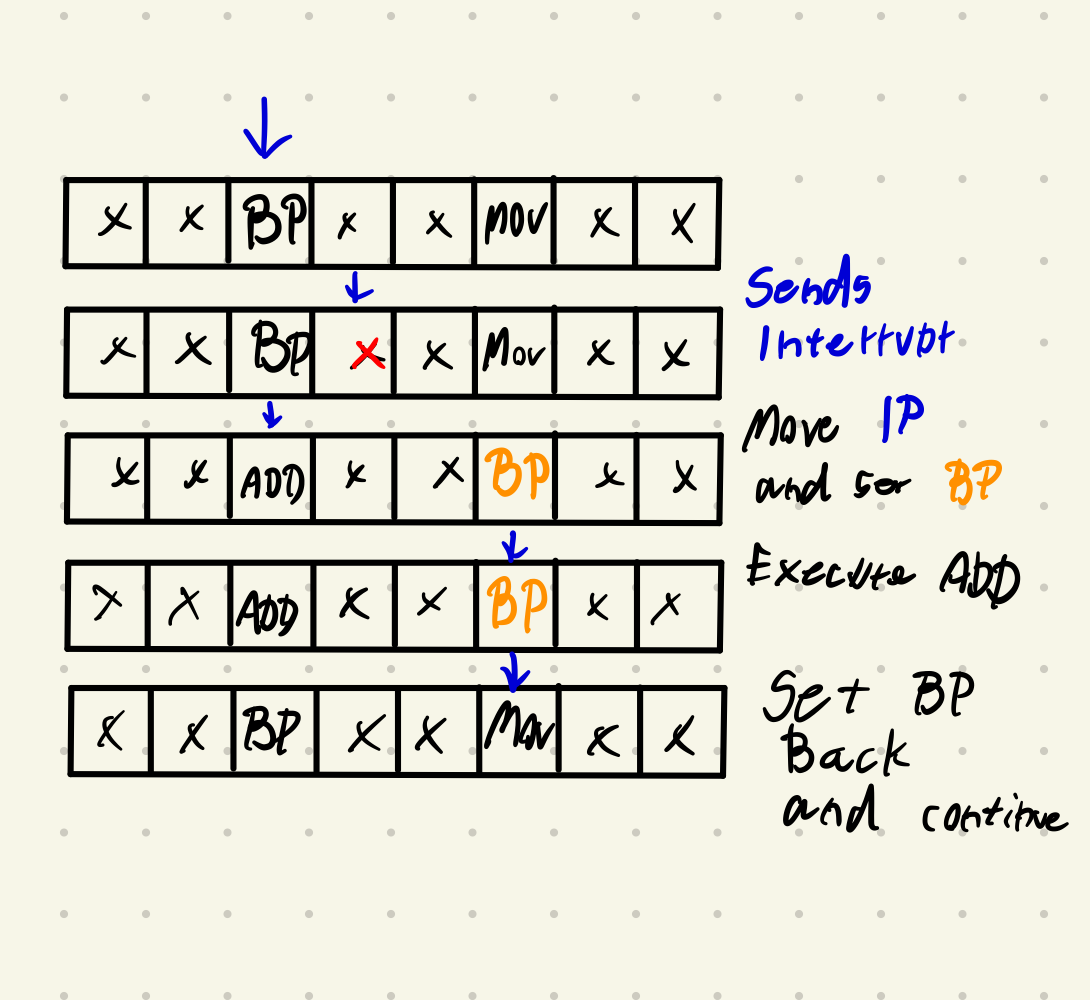
\includegraphics[width=100mm,scale=0.5]{media/breakpoint_tbd}
    \caption{Continue sketch}
\end{figure}

However, before we get to registers, we showed that the breakpoint must be put
at the next instruction. This is not as simple as it sounds. Where is next
instruction? On CISC architectures, this is not easy to find out since
instructions have different sizes. But even on RISC architectures like ARM,
what if the instruction is a jump of some sort and the next instruction is not
simply the one that follows this one in the code? For this reason, debuggers may
need to have an instruction emulator, which needs to emulate whole instruction
set to see where the program counter ends up\footnote{And there can be a
\textit{lot} of instructions \cite{intel-manual}}. However, some architectures
offer hardware support, like the trap flag we mentioned in section \todo{ref}.

The ptrace library contains special \texttt{PTRACE\_SINGLESTEP} command. This
executes one instruction in the tracee and then signal \texttt{SIGTRAP} will be
sent to it. The linux kernel (as of v6.1.8) uses previously mentioned trap flag
for x86 \cite{linuxkernel-trapflag}. If the architecture does not provide a way
to support single stepping then the call will return an error.

Registers themselves are simple like memory. Linux contains predefined structure
\texttt{user\_regs\_struct}, which maps all registers on current architecture.
The command \texttt{PTRACE\_GETREGS} then fills up this structure with the
value in registers.



\subsection{Windows}
Windows also has built-in support for debugging at the Win32API layer
\cite{windows-msdn-debugging-api, windows-press-debugging-api}.
It builds on \textit{debug events} and \textit{debug functions}. Summary of
some of the functions that Win32 API offers which all help with debugging:

\begin{itemize}
    \item \mintinline{c}{DebugActiveProcess} - Attaches the debugger to an active process.
    \item \mintinline{c}{DebugBreakProcess} - Causes a breakpoint exception to occur in the specified process.
                                          This passes control of the process to the debugger if there is one.
    \item \mintinline{c}{WaitForDebugEvent} - Waits for new debug events.
    \item \mintinline{c}{ContinueDebugEvent} - Continue the process execution after processing debug event.
    \item \mintinline{c}{OutputDebugString} - Sends a string to the debugger for display.
    \item \mintinline{c}{ReadProcessMemory} and \mintinline{c}{WriteProcessMemory} - Read and modify
          process virtual address space.
    \item \mintinline{c}{FlushInstructionCache} - Flushes instruction cache of the process.
\end{itemize}

The general structure of Windows debugger can be seen in figure \ref{fig:win32debugger}.
The debugger waits for debug events via function \mintinline{c}{WaitForDebugEvent}.
This function has a timeout parameter, so the debugger can also do other things while it's waiting.
These events are put in a queue, so the debugger will not miss any.

\begin{figure}
    \centering
    \scalebox{0.8}{
    \begin{tikzpicture}
        \draw (-7,0) -- (-7,-11) (0,0) -- (0,-11) (7,0) -- (7,-11);
        \node at (-7,.3) {Debugee};
        \node at (0,.3) {Win32 API};
        \node at (7,.3) {Debugger};
        \draw[<-] (0,-1) -- node[midway,above] {\mintinline{c}{CreateProcess}} (7,-1);
        \draw[<-] (-7,-2) -- node[midway,above] {Create} (0,-2);
        \draw[->] (0,-3) -- node[midway,above] {\mintinline{c}{CreateProcess} returns} (7,-3);
        \draw[<-] (0,-5) -- node[midway,above] {\mintinline{c}{ContinueDebugProcess}} (7,-5);
        \draw[<-] (0,-6) -- node[midway,above] {\mintinline{c}{WaitForDebugEvent}} (7,-6);
        \draw[dashed,->] (-7,-6.5) -- node[midway,above] {Exception} (0,-6.5);
        \draw[->] (0,-7) -- node[midway,above] {\mintinline{c}{WaitForDebugEvent} returns \texttt{true}} (7,-7);
        \draw[dashed, <-] (-7, -8) -- node[above left] {Debugger actions} (7, -8);
        \draw[<-] (0,-9) -- node[midway,above] {\mintinline{c}{ContinueDebugProcess}} (7,-9);
        \draw[<-] (0,-10) -- node[midway,above] {\mintinline{c}{WaitForDebugEvent}} (7,-10);
        \draw[dashed,->] (-7,-10.5) -- node[midway,above] {Exception} (0,-10.5);
    \end{tikzpicture}
    }
    \caption{A sequence diagram for debugger using Windows api. Inspired by \todo{NI-REV 6. lecture}}
    \label{fig:win32debugger}
\end{figure}

The debug events are thoroughly described in subsection \ref{section:Debug Events}. The main point of interest is the exceptions.
By these, we do not mean the standard C++ exceptions but rather Microsoft \textit{Structured Exception Handling}.

\subsubsection*{Debug Events}\label{section:Debug Events}
Debugging events are various incidents in the debuggee that causes the system
to notify the debugger \cite{windows-msdn-debug-events}. These are stored in
special \mintinline{c}{DEBUG_EVENT} structure, which is received in
\texttt{WaitForDebugEvent} call from debugger. This structure contains various
information about the event, the internals can be seen on figure
\ref{fig:DebugEvent}. These events include loading and unloading a DLL,
creating and exiting a process, sending debug strings via the
\mintinline{c}{OutputDebugString} and so on. It also includes exceptions, those
are probably the most important for us. 

\begin{figure}
\begin{minted}{c}
typedef struct _DEBUG_EVENT {
  DWORD dwDebugEventCode;
  DWORD dwProcessId;
  DWORD dwThreadId;
  union {
    EXCEPTION_DEBUG_INFO      Exception;
    CREATE_THREAD_DEBUG_INFO  CreateThread;
    CREATE_PROCESS_DEBUG_INFO CreateProcessInfo;
    EXIT_THREAD_DEBUG_INFO    ExitThread;
    EXIT_PROCESS_DEBUG_INFO   ExitProcess;
    LOAD_DLL_DEBUG_INFO       LoadDll;
    UNLOAD_DLL_DEBUG_INFO     UnloadDll;
    OUTPUT_DEBUG_STRING_INFO  DebugString;
    RIP_INFO                  RipInfo;
  } u;
} DEBUG_EVENT, *LPDEBUG_EVENT;
\end{minted}
\caption{Structure which contains info about debug event.}
\label{fig:DebugEvent}
\end{figure}

\subsubsection*{Structured Exception Handling}
This feature is specific to Windows only. For example, if division by zero was
performed in a program on Linux, a signal would be sent to the process. Windows
don't have signals, instead, it uses Structured Exception Handling
\cite{windows-msdn-seh}. From now on, we will be using the abbreviation 'SEH'.
An exception is an event that requires execution of code outside the normal
flow of control. There are software exceptions, like throwing an exception
explicitly or by OS, and hardware exceptions, like the division by zero we
mentioned. Instruction with opcode \mintinline{c}{0xCC}, which is used for
breakpoints, will also raise an exception. SEH unifies both of these things
into one.

When an exception is triggered, control is transferred to the system. It saves
the state of the thread and some other information. This information can be
used to continue execution from the point where the exception was thrown when
it is resolved. It also contains information about which type of exception was
thrown, if execution can continue after handling the exception, address where
the exception occured and some others\footnote{See MSDN documentation
\cite{windows-msdn-seh} for full detailed list}. The system then searches for
an exception handler which will handle the exception. The search is performed
in this order:

\begin{enumerate}
    \item If the process is debugged the debugger is notified.
    \item If it is not or the debugger does not handle the exception, the frame-based exception handler is to be found\footnote{The handlers are not very important to us, see MSDN documentation if you're interested \cite{windows-msdn-seh}.}
    \item If no frame-based handler can be found, or no handler handles the exception, but the process is being debugged then the debugger gets notified once again.
    \item The system provides default handling, which is to terminate the program via \mintinline{c}{ExitProcess} most of the time.
\end{enumerate}

Here we see that every exception that occurs in the debuggee causes the
debugger to be notified. Breakpoints are also caused by an exception, as was
briefly mentioned before. There are two possible notifications to the debugger.
The first is known as \textit{first-chance} notification
\cite{windows-msdn-dbg-exc-handling}. The debugger can (and should) inspect the
information about the exception and see if it was a breakpoint or single-step.
These only occurs if the process is debugged (it wouldn't happen otherwise) and
the debugger should handle them. If it is something else it can ignore the
exceptions. When the program is continued via
\mintinline{c}{ContinueDebugEvent}\footnote{This function has a special
parameter, which is used to tell that the exception was or was not handled.},
the debugger is notified once again if no appropriate exception handler was
found for the exception. This is known as \textit{last-chance} notification
because if the debugger does not handle the exception the debuggee will be
terminated. It gives the user a chance to debug why is his process terminating.

Here are some exceptions that tie into debugging:
\begin{itemize}
    \item \mintinline{c}{STATUS_BREAKPOINT} - Raised when a hardware-defined breakpoint was encountered. This includes the mentioned \mintinline{c}{INT3} instruction.
    \item \mintinline{c}{STATUS_SINGLE_STEP} - Raised when a single step was completed, ie. when instruction was executed and the trap flag is set.
\end{itemize}

\subsubsection*{Tying it all together}
Now we have all necessary building block to build a simple proof of concept
Windows debugger. On figure \ref{fig:windows-debugger-mainloop}, you can see a
basic idea of a main loop of the debugger. It waits for debug events and
branches depending of the type of event. It needs not only handle exceptions,
but other events also. For example if the debugee creates a thread that is
something the debugger should be aware of. Modern debuggers trace all threads
of the program.

\todo{Pridat dalsi figure kde je jak se hanndlujou tyhle blbosti} However,
exceptions are the most interesting for us. There, breakpoint and single step
handling should be done. On both of these, the debugger should handle the
exception itself, so this is the \textit{first chance} notifications. There is
also an \mintinline{DBG_CONTROL_C}, which happens on CTRL + C keyboard press.
This should terminate the program. The debugger will pass the first chance and
catch the last chance exception, so user has a final chance to look at the
program state before it exits.

\begin{figure}
    \begin{minted}{c}
void EnterDebugLoop(const LPDEBUG_EVENT DebugEv)
{
   DWORD dwContinueStatus = DBG_CONTINUE; // exception continuation
   for(;;)
   {
      WaitForDebugEvent(DebugEv, INFINITE);
      switch (DebugEv->dwDebugEventCode)
      {
         case EXCEPTION_DEBUG_EVENT:
            // Handle exception debug events
         // Other debug events
      }
   ContinueDebugEvent(DebugEv->dwProcessId,
                      DebugEv->dwThreadId,
                      dwContinueStatus);
   }
}
\end{minted}
\caption{Windows debugger main loop}
\label{fig:windows-debugger-mainloop}
\end{figure}

\section{Compiler support}
\todo{Moved from introduction here for the time being}
When we talked about evolution of programming from machine code to assembly to
higher level languages, we haven't talked about how they are executed. Machine
code can be directly executed by processor, as we said, it is a sequence of
binary. Assembly is text, processors don't understand text. But assembly can be
mapped to machine code almost 1:1\footnote{There are some exceptions, like
labels. But translating them is not very difficult.}.

However, high level programming languages do not map 1:1 to assembly. Some are
close to it, like C, while others are miles away, like Haskell. But as was
said, processors understand only machine code. To this end, programs that can
translate source code into machine code, were created. They are called
compilers and the translation process is called compiling. For example, for the
C language one might use the GCC or Clang compilers. On figure
\ref{fig:compiler-structure} can be seen basic structure of a compiler
\cite{dragon-book}. 

\tikzstyle{compilerblock} = [rectangle, draw, minimum width=6cm, minimum height=1cm] 
\tikzstyle{tables} = [rectangle, draw, minimum width=4cm, minimum height=1cm] 
\begin{figure}\label{fig:compiler-structure}
    {\centering
    \begin{tikzpicture}
    \node (lexer)[compilerblock]{Lexical analyzer};
    \node (syntax)[compilerblock,below=of lexer]{Syntactic analyzer};
    \node (semantic)[compilerblock,below=of syntax]{Semantic analyzer};
    \node (imc)[compilerblock,below=of semantic]{Intermediate Code Generator};
    \node (gen)[compilerblock,below=of imc]{Code Generator};
    \node (symbol)[tables, left=of semantic]{Symbol table};
    \draw[->] (lexer) -- node[below] {} (syntax);
    \draw[->] (syntax) -- node[below] {} (semantic);
    \draw[->] (semantic) -- node[below] {} (imc);
    \draw[->] (imc) -- node[below] {} (gen);
    \end{tikzpicture} 
    \par}
    \caption{Simplified structure of a compiler. Some parts were left out, like optimizations.}
    \label{fig:compiler_tikz}
\end{figure}

\subsection{Lexical analyzer}
The lexical analyzer groups separate symbols into groups. For example the code
\begin{minted}{c}
foo = bar(1 + 2);
\end{minted}
might be translated into tokens like this
\begin{lstlisting}[stringstyle=\color{black}]
<id:"foo"> <assignment-operator> <id:"bar"> 
<left-bracket> <int-number:1> <plus-operator> 
<int-number:2> <right-bracket> <semicolon>
\end{lstlisting}
The Syntactic analyzer then works with these tokens.

\subsection{Syntantic and semantic analyzer}
Syntactic analysis accepts tokens and processes them into other intermediate
representation. This is most often an abstract syntax tree (abbr. AST, figure
\ref{fig:ast}). It also checks that the source code complies to the grammar of
the language. Semantic analysis then checks that the program is semantically
consistent. For example that used variable has been declared before.

\begin{figure}\label{fig:ast}
    \centering
    \begin{tikzpicture}[,shorten >=1pt,node distance=1.8cm,on grid,initial/.style={}]
    \node (assignment) {$=$};
    \node (foo) [below left =of assignment] {id:foo};
    \node (bar) [below right =of assignment] {call:bar};
    \node (plus) [below right=of bar] {$+$};
    \node (one) [below left =of plus] {$1$};
    \node (two) [below right =of plus] {$2$};
    
    \draw[-, above, scale=0.7] 
    (assignment)   edge node[scale=0.7, left, yshift=0.1cm] {lhs}  (foo)
     (assignment)  edge node[scale=0.7, right, yshift=0.1cm] {rhs}  (bar)
     (bar)         edge node[scale=0.7, right, yshift=0.1cm] {expr} (plus)
     (plus)        edge node[scale=0.7, right, yshift=0.1cm] {rhs}  (two)
     (plus)        edge node[scale=0.7, left, yshift=0.1cm] {lhs}  (one);
    \end{tikzpicture}
    \caption{Simplified example of an abstract syntax tree.}
    \label{fig:astgraph}
\end{figure}
 
\subsection{Intermediate code generation}
This part converts AST into some other representation, most commonly called
IR\footnote{IR means intermediate representation. AST is also intermediate
representation, but if we use IR we mean this one.}. IR is closer to machine
code, to be easily translated, but retain some properties that makes it easier
to work with it. There are many types of IR. One of the most popular compilers,
LLVM, uses single static assignment (SSA) \cite{llvm}. Example of LLVM IR can
be found on figure \ref{fig:llvm-ir-example}. Compilers perform most
optimizations on this intermediate representation. 

\begin{figure}\label{fig:llvm-ir-example}
    \begin{minted}{llvm}
        define dso_local i32 @_Z6squarei(i32 %0) {
          %2 = alloca i32, align 4
          store i32 %0, i32* %2, align 4
          %3 = load i32, i32* %2, align 4
          %4 = load i32, i32* %2, align 4
          %5 = mul nsw i32 %3, %4
          ret i32 %5
        }
    \end{minted}
    \caption{Simplified example of LLVM IR.}
\end{figure}

\subsection{Code generation}
Here, IR is translated directly to the target machine code or possibly
assembly. Even though IR can seem very similar to assembly, there are still
some things to take care of. For example SSA IR doesn't have registers, it uses
unlimited number of variables. Other architectures might have some other traits
that differ it from the IR and they all have to be accounted for when
generating code.

\subsection{Modularity of compilers}
The main advantage of using an IR is that there is a common ground for every
language. Imagine we write a compiler for the C language. We need to write all
five parts from figure \ref{fig:compiler-structure}. If we later decided that
we also want to create a compiler for Haskell, we just need to write everything
up to the IR translation. Once we can translate Haskell into the IR, we can
reuse the previous part of the compiler to compile to machine code! This also
works the other way around. If we compiled IR to the machine code that works
with the x86 architecture, and we want to compile to ARM, we just need to
create the code generation part for the ARM architecture, no need to write
whole compiler. Also, most of the optimizations are done on the IR level, this
also saves a lot of development time. The parts of the compiler which are
dependent on the source language are called \textbf{frontend} (Syntax, Semantic
and IR translation), the parts that are dependent on the target are called
\textbf{backend} (Code generation).

This is widely used in practice. The LLVM \cite{llvm} project is a compiler
backend. It uses its own IR (as was mentioned on figure
\ref{fig:llvm-ir-example}). It can compile this IR into many targets, including
x86, ARM and Spark \todo{Ocitovat}. The \textit{Clang} project is a compiler
frontend for C, C++ and Objective-C languages. It translates these languages to
the LLVM IR. Other frontends for LLVM also include \textit{ghc}, which is a
Haskell compiler, or \textit{rustc}, which is a Rust compiler. With LLVM,
creating new programming language comes down to parsing it into an AST and
transforming that AST into the LLVM IR.

\subsection{Interpreting programs}
Not all languages are compiled. Imagine a program which can evaluate arithmetic
expressions, each phone nowadays has a program like this. We don't have to stop
there. Moving this up a notch, we can create a program that reads source code
and executes it. This is what interpreting means. Dynamically typed languages
tend to be interpreted~\cite{python, lua, javascript}\todo{Instead of
languages, cite some relevant source}, but it is not a rule~\cite{scala}. Since
the interpreter is a program, it is another layer of abstraction. This can make
the resulting languages sometimes more abstract then the compiled ones,
sometimes at the cost of performance~\cite{jit}. Interpreters still
\textit{compile} the code into some intermediate representation, but it's not
compiled down to machine code, instead that IR is run by a
program\footnote{Nowadays, interpreters use JIT compilation, which compiles
some of the code some of the time into machine code~\cite{jit}}.

\chapter{Tiny86}\label{section:T86}
At the FIT CTU, in the NI-GEN course, students have to write a compiler. The
Tiny86 (T86) architecture was created to make code generation easier. This
allows the students to focus on more interesting parts of compiler design, such
as optimizations. To be able to execute programs written using this
architecture, a virtual machine was created. This was all done as a part of a
master's thesis made by Ivo Strejc~\cite{ivo2021tiny}. This chapter explores
said architecture and the virtual machine. It also delves into the existing
debugging capabilities of said virtual machine.

\section{The T86 Instruction Set Architecture}
The T86 name is an abbreviation for Tiny x86. It was designed with a goal in
mind, that goal being the fact that it is an educational ISA. The Virtual
Machine made for the ISA allows configuring the number of registers, the RAM
size, or the length of each instruction. This allows the student to develop
their compilers incrementally.

The T86 uses a Harvard architecture, meaning the data and instructions are
physically separated. The author doesn't specify the reason for this.
Presumably, it is to ease the implementation of the virtual machine since the
memory and instructions can be represented as two separate array-like members
of the virtual machine. Memory is addressable by 64-bit blocks, not by 8-bit
blocks as is the custom in modern computers.

It shares some of the registers we saw on x86-64: the program counter (PC), the
stack pointer (SP), the base pointer (BP), and the flags register. The intended
roles for these registers are the same as on x86-64 architecture. It also has
other general-purpose registers. As previously said, the amount of these is
configurable. The registers store a 64-bit value. It also has float registers,
which can store 64-bit float values. These are separated from the standard
registers, similarly to x86-64.

The addressing modes, or what kind of operands instructions can have, include
immediate values, registers, and memory accesses. They can also be combined in
various ways, like \texttt{[R0 + R1 * 2]}, or \texttt{[R0 + 10 + R1 * 2]}. The
addressing modes are, however, not arbitrary, \texttt{[R0 + R1 + R2]} is not a
correct addressing mode for T86. For a full list, refer to \cite{ivo2021tiny}.
The instructions that are taken over from x86-64 have more restrictive
addressing modes than in x86-64. For example, the \verb|add| instruction can
take a memory offset as a destination operand in x64-86, but in T86, it can
only take registers.

Other than that, the ISA is a subset of the x86-64 most used instructions, many
of which we have already seen in various examples throughout the thesis.
Interesting exceptions are the IO instructions - \texttt{PUTCHAR} and
\texttt{GETCHAR}, which allow for very primitive input and output handling.
Also, an \texttt{DBG} and \texttt{BREAK} are defined. These are used for
debugging, but in a very different way than we have seen in previous sections.
We will touch upon them when discussing the virtual machine implementation
since they are very much tied to it. A small sample of a T86 program can be
seen in figure \ref{fig:t86-example}.

\begin{figure}
    \begin{lstlisting}
SUB SP, 1
MOV R0, 5
MOV [BP - 2], R0
LEA R1, [BP - 2]
MOV [BP - 1], R1
MOV R2, 4
    \end{lstlisting}
    \caption{A small piece of a T86 program.}
    \label{fig:t86-example}
\end{figure}

\subsection{T86 Virtual machine}\label{section:t86-vm}
The primary objective of the virtual machine is to replicate the CPU as
accurately as possible, without prioritizing execution speed. For instance, the
virtual machine simulates the out-of-order technique briefly described in
section \ref{section:superscalar-cpu}. The purpose of the virtual machine is to
allow the students to gain a deeper understanding of the effects of pipeline
stalls and similar events on program speed. The virtual machine is able to
generate statistics that provide information about these factors and how
much they influenced the speed of the generated program.

The virtual machine (VM) is implemented in C++, using the newer standards up to
C++17. The VM offers only a single interface, and that is the
\texttt{ProgramBuilder}. This is a class through which one may construct a
program for the T86 VM. An example of how to use this class is in figure
\ref{fig:t86-intro}. Currently, there is no other way for users to run programs
in the VM. This means that the students are tied to the C++ language, or use
some bindings if they want to use other language.

\begin{figure}
    \begin{minted}{cpp}
        ProgramBuilder pb;
        pb.add(MOV{Reg(0), 50);
        pb.add(PUTCHAR{Reg(0)});
        pb.add(HALT{});
        auto program = pb.program();
        Cpu cpu;
        cpu.start(std::move(program));
        while (!cpu.halted())
        cpu.tick();
    \end{minted}
    \caption{Simple example of how to create and run a simple program in the T86 VM.}
    \label{fig:t86-intro}
\end{figure}

\subsubsection{Debug instructions}\label{section:t86-debug-cap}
The VM offers some limited debug capabilities. It has the \texttt{DBG} and
\texttt{BRK} instructions. The \texttt{DBG} instruction takes as an operand a
function. The function has the following signature: \texttt{void fun(Cpu\&)}.
This function then gets executed when the instruction is hit. This can prove
helpful in inspecting the internal state of the CPU. In figure
\ref{fig:t86-debug}, we show a possible usage of this instruction. The
\texttt{BRK} instruction works similarly. It, however, has no operand. Instead,
a function must be provided before execution to the CPU itself. \texttt{BRK}
then always runs this function when hit.

\begin{figure}
    \begin{minted}{cpp}
    pb.add(DBG{[](Cpu& cpu) {
        if (cpu.getRegister(Reg{0}) == 0) {
            std::cerr << "Register 0 is set to zero!\n";
        }
    });
    \end{minted}
    \caption{Example of an debug instruction in T86 VM.}
    \label{fig:t86-debug}
\end{figure}

Such debugging capabilities can be helpful but quickly prove insufficient. For
example, when a step-by-step inspection is sought, a debug instruction must be
placed at every second line of the program. Also, interactivity is not present.
However, this function can accept input, so one could create a robust enough to
handle register and memory writing. An idea of how this could be done is
illustrated in \ref{fig:t86-pocket-debugger} via the \texttt{BRK} instruction.

\begin{figure}
    \begin{minted}{cpp}
    cpu.connectBreakHandler([](Cpu& cpu) {
        char command;
        std::cin >> command;
        if (command == 'c') return; // continue
        else if (command == 'r') { // Read register
            int num;
            std::cin >> num;
            int regval = cpu.getRegister(num);
            std::cerr << std::format("Register {} = {}\n",
                                     num, regval);
        } else if (command == 'w') { // Write register
            int num;
            int val;
            std::cin >> num >> val;
            cpu.setRegister(Reg{num}, Reg{val});
        }
        ... // Other commands
    });
    \end{minted}
    \caption{Small debugger implementation using T86 BRK instruction, abbreviated.}
    \label{fig:t86-pocket-debugger}
\end{figure}

This still leaves much to be desired. Not to mention placing the debug
instruction can prove very bothersome.

\chapter{Implementation}
In this chapter, we describe how we went about the implementation
of the debugger and reason about the design choices we made.
Also, we describe which part of the virtual machine were
modified or added for the benefit of the debugger or in
general for the greater good.

\section{T86 ISA extensions}\label{section:parser}
In chapter \todo{ref} we showed how to build a program for the T86 VM. It was
necessary to use the builder the T86 VM provides. There is currently no other
way. We remedied this with a hand-made parser of the T86 assembly language. An
example of a program for T86 is shown in figure \ref{fig:t86-program}. It is
very similar to assembly we have shown in previous sections. Thanks to this,
students can choose any language they want to implement their compiler and just
emit this assembly at the end. An unfortunate side effect is that we are no
longer able to use the \texttt{DBG} instruction. This will however be remedied
by the very debugger we are implementing here. 

Notice the \texttt{.text}, this is a section, same as the ELF format uses. We
will carry some of this over from the ELF format. Mainly, the \texttt{.text}
and \texttt{.data} sections. For debugging purposes, we will also include some
debug headers. The exact nature of this debugging headers is specified in
section \todo{ref} where the debugging information format for our debugger is
defined.

\begin{figure}
    \begin{lstlisting}
        .text

        0 MOV R0, 49
        1 PUTCHAR R0
        # Put newline
        2 MOV R0, 10
        3 PUTCHAR R0
        4 HALT
    \end{lstlisting}
    \caption{Example of an T86 program.}
    \label{fig:t86-program}
\end{figure}

We will also add a few new instructions. One is \texttt{PUTNUM}, which prints
the numerical value with a newline. This is intended as a simple debug instruction
and to ease the automated testing of the compiler. Only other way of output was
to print a char which was represented by the ascii value. If students wants
to have an automated test that his factorial program translates successfully
it is very much easier with this instruction.

Another one is the \texttt{BKPT} instruction. This instruction is similar to
\texttt{INT3} from x86\_64 or \texttt{BKPT} from ARM. It is an software
breakpoint. When the instruction is hit, a control will be passed to the
connected debugger. This is thoroughly described in the next section. 

\section{Design of the native T86 debugger}
We could simply bake the debugger into the virtual machine itself. This would
probably prove to be simplest to implement. However, the main point of the
debugger is not only to ease the code generation part, but to be a learning
point so that students might grasp how a real debugger is
implemented\footnote{The VM followed the same philosophy.}. Because of this, we
aim to simulate the real world debuggers as close as possible. The compilers
themselves may also have more targets in the future, not just the T86 VM. If we
made the debugger as part of T86 we couldn't use it for a possibly new virtual
machine. In conclusion, the virtual machine and the debugger will be two
entirely different programs, and as such, two completely different processes.

In the implementation of debugger for Linux, which was the subject of section
\todo{ref}, we described how the kernel of an operating system helps with the
implementation of the debugger via specific API. There is no operating system
between the virtual machine and the program. Still, we will strife to make the
API similar on the virtual machine part. The debugger and the VM will have to
communicate together somehow. For the interprocess comunnication, there are
several possibilities.

One of those are signals. Those however are POSIX specific. Other possibilities
are shared pipes or sockets. We choose sockets, purely because \todo{we do not
known how to use anything else :)}. Both the virtual machine and the debugger
will have an opened port through which they will communicate. The format
of the communication will be a text one, merely because of the ease of use
as opposed to binary format. The commands that the virtual machine API
will offer are
\begin{itemize}
    \item \texttt{READREG x} - Return value in register \texttt{x}.
    \item \texttt{WRITEREG x y} - Sets the value in register \texttt{x} to \texttt{y}.
    \item \texttt{READDATA x} - Return value in memory at address \texttt{x}.
    \item \texttt{WRITEDATA x y} - Writes a value \texttt{y} into a memory at address \texttt{x}.
    \item \texttt{GETTEXT x} - Returns instruction at address \texttt{x}.
    \item \texttt{WRITETEXT x} \texttt{INS} - Rewrite the instruction at address
        \texttt{x} with the newly supplied instruction.
    \item \texttt{CONTINUE} - Continue the execution.
    \item \texttt{REASON} - Get the reason why the program stopped (breakpoint, singlestep, halt).
    \item \texttt{SINGLESTEP} - Does native level single step.
\end{itemize}
Example of how those commands can be used for communication between the virtual
machine and the debugger is shown in figure \ref{fig:dbg-vm-seq}. The interface
is similar to basic ptrace commands. We separate the memory and instruction
writing because T86 use harvard architecture, whereas Linux doesn't separate
text and data address spaces, so the two requests were equivalent there.

Currently, the class that runs the program is the \texttt{Cpu}. We will add
another manager-like class. This class will take care of running the program
via the \texttt{Cpu} class and it will also manage said debugger requests. The
\texttt{Cpu} class will return control to the manager when a reason for
stopping happens. We will call these reasons \textit{interrupts} because they
are somewhat similar to real world CPUs interrupts. The manager is then
responsible for dealing with the interrupt and handling control back to the
\texttt{Cpu} or terminating the program.

The \texttt{Cpu} does not have a way to modify the instruction vector.
However, we can leverage our previously implemented parser from section
\todo{section:parser}and create the instruction on the fly.

\begin{figure}
    \centering
    \scalebox{0.8} {
    \begin{tikzpicture}
        \draw (0,0) -- (0,-17.2) (7,0) -- (7,-17.2);
        \node at (7,.3) {Debugger};
        \node at (0,.3) {Virtual machine};
        \draw[<-] (0,-1) -- node[midway,above] {Initializes connection} (7,-1);
        \draw[->] (0,-2) -- node[midway,above] {Accepts connection} (7,-2);
        \draw[<-] (0,-3) -- node[midway,above] {\texttt{READINS 5}} (7,-3);
        \draw[->] (0,-4) -- node[midway,above] {Ok} (7,-4);
        \draw[<-] (0,-5) -- node[midway,above] {\texttt{WRITEINS 5 BRKPT}} (7,-5);
        \draw[->] (0,-6) -- node[midway,above] {Ok} (7,-6);
        \draw[<-] (0,-7) -- node[midway,above] {\texttt{CONTINUE}} (7,-7);
        \draw[->] (0,-8) -- node[midway,above] {Ok} (7,-8);
        \draw[->] (0,-10) -- node[midway,above] {Program stopped} (7,-10);
        \draw[<-] (0,-11) -- node[midway,above] {\texttt{REASON}} (7,-11);
        \draw[->] (0,-12) -- node[midway,above] {Reason: \texttt{BKPT} instruction} (7,-12);
        \draw[<-] (0,-13) -- node[midway,above] {\texttt{CONTINUE}} (7,-13);
        \draw[->] (0,-15) -- node[midway,above] {Program stopped} (7,-15);
        \draw[<-] (0,-16) -- node[midway,above] {\texttt{REASON}} (7,-16);
        \draw[->] (0,-17) -- node[midway,above] {Reason: \texttt{HALT} instruction} (7,-17);
    \end{tikzpicture}
    }
    \caption{A sequence diagram for the virtual machine and debugger communication.}
    \label{fig:dbg-vm-seq}
\end{figure}



\begin{conclusion}
	Conclusion text yet to be concluded.
\end{conclusion}

\bibliographystyle{iso690.bst}
\bibliography{ref}

\appendix

% \printglossaries

\chapter{Contents of CD}\label{app:CDcontent}

Visualise the contents of enclosed media. Use of \verb|dirtree| is recommended. Note that directories src and text with appropriate contents are mandatory.

\begin{figure}
	\dirtree{%
		.1 readme.txt\DTcomment{the file with CD contents description}.
		.1 data\DTcomment{the data files directory}.
		.2 graphs\DTcomment{the directory of graphs of experiments}.
		.3 *.eps\DTcomment{the B/W graphs}.
		.3 *.png\DTcomment{the color graphs}.
		.3 *.dat\DTcomment{the graphs data files}.
		.1 exe\DTcomment{the directory with executable WBDCM program}.
		.2 wbdcm\DTcomment{the WBDCM program executable (UNIX)}.
		.2 wbdcm.exe\DTcomment{the WBDCM program executable (Windows)}.
		.1 src\DTcomment{the directory of source codes}.
		.2 wbdcm\DTcomment{the directory of WBDCM program}.
		.3 Makefile\DTcomment{the makefile of WBDCM program (UNIX)}.
		.2 thesis\DTcomment{the directory of \LaTeX{} source codes of the thesis}.
		.3 figures\DTcomment{the thesis figures directory}.
		.3 *.tex\DTcomment{the \LaTeX{} source code files of the thesis}.
		.1 text\DTcomment{the thesis text directory}.
		.2 thesis.pdf\DTcomment{the Diploma thesis in PDF format}.
		.2 thesis.ps\DTcomment{the Diploma thesis in PS format}.
	}
\end{figure}


\end{document}
